\documentclass[tikz, border=4pt]{standalone}

% --- packages (mirror these in v-source.meta.json "requires") ---
\usepackage{tikz}

% --- palette (canonical source: reference/color-palettes/color-palettes.md; light variant) ---
% --- ESL domain-semantic tokens (contract §2, ADR-0005 D7) ---
\colorlet{inputdomain}{blue}

\begin{document}
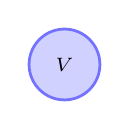
\begin{tikzpicture}
  % contract §1a `v-source`: "input voltage / activation source" -- the
  % hand-styled family node (not a circuitikz bipole; see esl-crossbar-kcl's
  % `vsource` style, which this icon is the standalone form of).
  \node[circle, draw=inputdomain!55, line width=1pt, fill=inputdomain!18,
        minimum size=9mm, inner sep=0pt, font=\scriptsize\itshape] (v) {$V$};
\end{tikzpicture}
\end{document}
